\section{Internetworking}
Una inter-network è una rete che mette in collegamento altre reti: \emph{è una rete di reti}.
Ognuna delle reti che partecipa usa tecnologie diverse, diverse caratteristiche fisiche, diversi formati dei frame e diversi schemi di indirizzamento.

\begin{figure}[H]
    \centering
    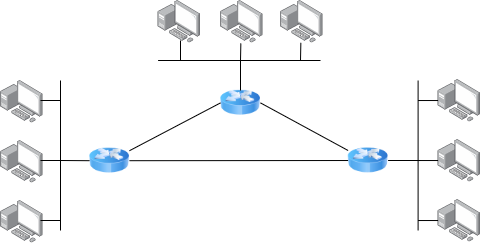
\includegraphics[width=200px]{images/5_Internetworking/inter-network.png}
\end{figure}

A fare la traduzione tra due o più reti c'è un interprete detto \emph{router} che si occupa di parlare queste "lingue diverse" e permettere il transito delle informazioni.

Per permettere questa interoperabilità creiamo un altro layer che ci permetta di creare l' astrazione che tutte queste reti diverse siano una singola rete unica ed omogenea.
Il protocollo principale di internetworking per Internet è IP.

\subsection{Introduzione}
Permette il trasferimento in maniera trasparente dei pacchetti, \emph{datagram}, dal nodo sorgente al nodo destinatario attraverso le varie reti intermedie.
Dal lato sorgente incapsula i dati ricevuti dal layer di trasporto, al lato destinatario invia i dati ricevuti al livello di trasporto.

Questo protocollo deve essere implementato in tutti gli host ed anche nei router in quanto, appunto, devono provvedere al forward, quindi dovranno poter interpretare le informazioni presenti nell' header del datagramma.


\subsubsection{Routing \& Forwarding}
\begin{itemize}
    \item forwarding: muove i pacchetti dall' interfaccia di ingresso del router all' interfaccia di uscita corretta
    \item routing: determina il percorso ottimale da far seguire al pacchetto per farlo arrivare a destinazione.
    Prevede l' utilizzo di algoritmi di routing cercando di ottimizzare una o più metriche.
\end{itemize}

Per fare una analogia: il routing è il processo di pianificare un viaggio partendo da una sorgente ed una destinazione, il forwarding è il processo di seguire il percorso step-by-step.

Gli algoritmi di routing permettono di generare la tabella di forwarding che ci dice in base all' indirizzo di destinazione quale uscita prendere.
Il forwarding poi usa questa tabella per indirizzare i pacchetti.

\subsubsection{Tipi di servizio}
Discerniamo i tipi di servizio in base al tipo di connessione:
\begin{itemize}
    \item connectionless: ogni pacchetto è gestito individualmente, si dice protocollo a datagramma
    \item connection: si sceglie un percorso predefinito all' inizio, creando di fatto un canale di comunicazione. Questo canale va poi anche deallocato alla fine del trasferimento 
\end{itemize}

I processi connectionless sono più veloci in quanto non c'è la costruzione della connessione, tantomeno il teardown.
Inoltre ogni router deve anche mantenere in memoria meno informazioni non dovendo sapere come si compone il circuito.
I pacchetti possono poi prendere strade diverse, il che è positivo se la struttura della rete cambia o se alcuni link diventano più occupati di altri.

Nel caso dei datagrammi la complessità è spostata agli estremi della rete, nei protocolli a connessione la complessità è nella rete stessa.
La rete a datagrammi può adattarsi, è più flessibile e permette link di diversi tipi e caratteristiche.

\subsubsection{Modelli di servizio}
Alcuni servizi che sarebbe comodo avere potrebbero essere:
\begin{itemize}
    \item affidabilità nella consegna
    \item consegna in ordine
    \item garanzia per una banda minima e di un delay massimo
    \item security nei fronti di confidenzialità, integrità ed autenticazione
\end{itemize}
Il modello di servizio di Internet è conosciuto come \emph{best-effort} cioè si fa il minimo indispensabile per recapitare i dati.
Non ci garantisce niente di ciò che richiediamo, tuttavia ci permette di costruire tutte queste caratteristiche nei layer superiori.

\subsection{Architettura di un router}
Il router svolge due principali funzioni:
\begin{itemize}
    \item forwarding dei datagrammi
    \item eseguire algoritmi/protocolli di routing interfacciandosi con gli altri router della rete
\end{itemize}

\begin{figure}[H]
    \centering
    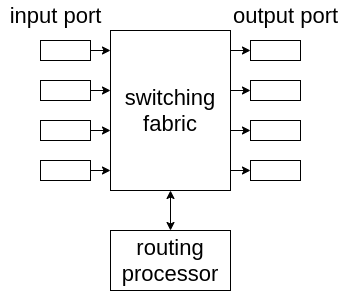
\includegraphics[width=200px]{images/5_Internetworking/router-architecture.png}
\end{figure}

\subsubsection{Porta di ingresso}
Deve "parlare" i primi 3 layer dello stack TCP/IP in quanto deve leggere i bit dal media, eseguire la error detection estrando il frame, successivamente estrarre il datagram IP.
Si guarda l' indirizzo di destinazione, si sceglie quale porta usare per rispedire il pacchetto e si inserisce il datagramma nel buffer interno della porta di uscita.
Se non è il primo datagram che arriva allora viene inserito nella coda della porta di ingresso finché non è il suo turno.

La commutazione tra ingresso e uscita può essere eseguita in modi diversi:

\begin{itemize}
    \item memoria condivisa:
    ogni interfaccia è costituita da un processore che ha accesso alla memoria come tutti gli altri
    \begin{figure}[H]
        \centering
        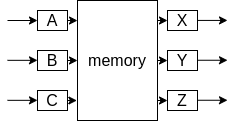
\includegraphics[width=150px]{images/5_Internetworking/memory.png}
    \end{figure}
    Non è molto performante a causa degli innumerevoli accessi alla memoria.

    \item via bus: i datagrammi vengono inviati su un bus condiviso tra tutte le interfacce.
    \begin{figure}[H]
        \centering
        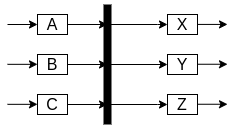
\includegraphics[width=150px]{images/5_Internetworking/bus.png}
    \end{figure}
    Anche questo approccio è lento perché bisogna gestire gli accessi al bus in mutua esclusione

    \item crossbar: un circuito più complesso che permette di collegare ogni interfaccia in ingresso con ogni interfaccia di uscita singolarmente
    \begin{figure}[H]
        \centering
        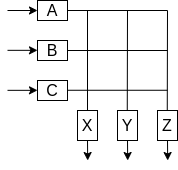
\includegraphics[width=150px]{images/5_Internetworking/crossbar.png}
    \end{figure}
    E' più complessa ma più efficiente
\end{itemize}

\subsubsection{Porta di uscita}
Questa interfaccia legge i dati dal suo buffer e provvede ad inviarli.
La coda può essere gestita in maniera arbitraria, non per forza First-Come-First-Served, si potrebbe ad esempio dare una priorità ad alcuni datagrammi che necessitano una qualità di servizio maggiore.

\subsection{Internet Protocol - IP}
E' di fatto il principale protocollo di livello Network, si serve tuttavia di informazioni generate da altri protocolli di livello rete.
Vediamo come si compone il datagramma IP (versione 4):
\begin{figure}[H]
    \centering
    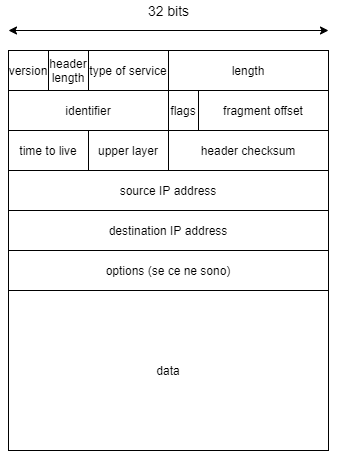
\includegraphics[width=200px]{images/5_Internetworking/ip_datagram_format.png}
\end{figure}

\begin{itemize}
    \item version: indica la versione del protocollo IP da usare (possiamo usare solo 4)
    \item header length: indica la dimensione dell' header in parole da 32 bit
    \item type of service: indica il quality of service dei dati che si stanno trasportando, usati per fare differenziazione del traffico e dare priorità
    \item length: lunghezza totale del datagramma
    \item identifier, flags, fragment offset: usati per la frammentazione
    \item time to live: indica il numero massimo di hop che il datagramma può ancora fare, ogni hop che riceve il pacchetto decrementa questo campo, una volta arrivato a 0 si droppa automaticamente e si notifica il nodo sorgente dell' accaduto 
    \item upper layer: indica il layer superiore al quale consegnare i dati di questo datagramma
    \item header checksum: checksum dell' header
    \item source IP address: indirizzo IP sorgente
    \item destination IP address: indirizzo IP destinatario
    \item options: informazioni aggiuntive sul pacchetto o sul forwarding come ad esempio (in genere non ci sono):
    \begin{itemize}
        \item source routing: si inseriscono gli hop sui quali instradare il pacchetto, indicando di fatto quale percorso deve seguire il pacchetto
        \item timestamp: si può aggiungere un timestamp nel pacchetto
    \end{itemize}
    \item data: dati da incapsulare provenienti dal layer superiore
\end{itemize}
E' necessario formulare un nuovo tipo di pacchetto per rendere interoperabili tutti i tipi di reti tra di loro, se usassimo il frame non ci sarebbe interoperabilità perché ogni rete definisce il suo modello di frame in base alla tecnologia ed il protocollo che usa, avendo questo formato invece possiamo rendere interoperabili tutte le reti in quanto per navigare all' interno della stessa rete usiamo frame, per navigare tra le diverse reti invece usiamo il formato IP.

\subsubsection{Frammentazione}
Un datagramma IP può essere grande al massimo 64Kbyte, la massima dimensione di un frame ethernet è di 1500 byte, non possiamo quindi inviare un datagramma IP usando un solo frame ethernet.
Si ricorre quindi alla frammentazione del datagramma cioè si divide il datagramma in porzioni più piccole inviate singolarmente e poi ricostituite alla ricezione.

Ogni frammento viene trattato come un datagramma quindi avrà lo stesso header di quello originale ma ora si popolano anche i campi per la frammentazione.
\begin{itemize}
    \item l' ID prende lo stesso ID del datagramma originale
    \item il fragment flag (more fragment bit) prende 1 se il datagramma non è l' ultimo, prende 0 se è l' ultimo da inviare
    \item L' offset prende il numero dei byte inviati fino ad ora e lo divide per 8. Questo perché non abbiamo 16 bit per questo campo ma solo 13, si indica quindi il punto nel datagramma originale nel quale inserire il frammento corrente piuttosto che il numero della posizione.
\end{itemize}

Supponiamo di voler inviare un datagramma da 5000 byte su un media che ha un MTU (max transmission unit) di 1500 byte, procediamo a frammentare:
\begin{figure}[H]
    \centering
    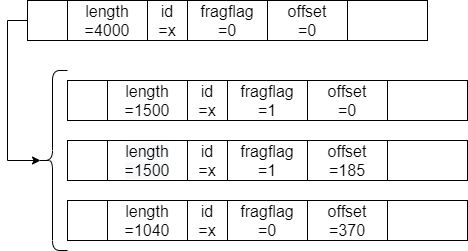
\includegraphics[width=300px]{images/5_Internetworking/fragmentation_example.png}
\end{figure}
\begin{itemize}
    \item tutti i frammenti prendono lo stesso id
    \item i primi due frammenti prendono il fragment flag ad 1, l' ultimo a 0
    \item il primo prende dimensione 1500byte (1480 di dati e 20 di header) ed offset 0
    \item il secondo prende dimensione 1500byte e come offset $\frac{byte\_inviati}{8} = \frac{1480}{8} = 185$
    \item il secondo prende dimensione 1040byte (i rimanenti) e come offset $\frac{2960}{8} = 370$
\end{itemize}
Se dopo aver frammentato un altro router trova un media con MTU ancora minore, può frammentare ancora di più.

Se ci accorgiamo che non abbiamo tutti i frammenti non possiamo fare altro che buttare tutto quanto e chiedere all' host sorgente di reinviare tutto quanto, questo perché non possiamo sapere chi ha eseguito la frammentazione quindi non sappiamo a chi chiedere.
Inoltre questo approccio è coerente con la filosofia best effort del protocollo.


\subsection{IP addressing}
Un  indirizzo IP è un valore composto da 32 bit ed identifica un host connesso nella rete, o meglio una interfaccia di un host connessa nella rete, solitamente si rappresenta e si legge in notazione decimale puntata.

Un indirizzo IP è detto strutturato in quanto si compone di due parti:
\begin{itemize}
    \item subnet part: i bit più alti
    \item host part: i bit più bassi
\end{itemize}
Una sottorete è l' insieme delle interfacce con la stessa porzione di sottorete nell' indirizzo IP che possono parlare tra di loro senza neanche l' utilizzo del router.
\begin{figure}[H]
    \centering
    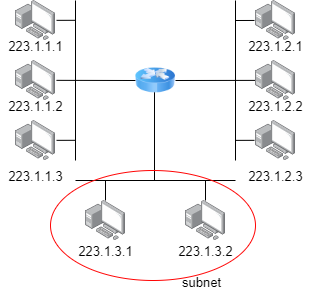
\includegraphics[width=200px]{images/5_Internetworking/subnet.png}
\end{figure}

Questa organizzazione è di tipo gerarchico, conoscendo la parte di rete di un indirizzo IP abbiamo informazioni che riguardano la posizione di un nodo in quanto tutti gli elementi di una stessa rete saranno connessi tra di loro.

\subsubsection{Classi degli indirizzi IP}
Suddividiamo gli indirizzi IP in alcune categorie:
\begin{figure}[H]
    \centering
    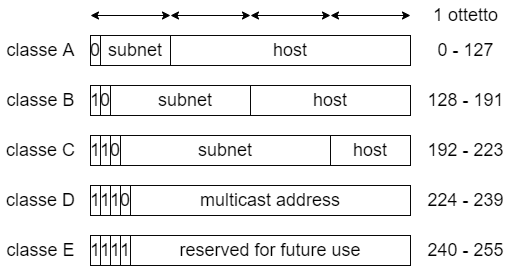
\includegraphics[width=300px]{images/5_Internetworking/ip_classes.png}
\end{figure}
Si noti che più bit di host ci sono e più host può accogliere una rete, ma meno reti ci possono essere di quel tipo, per esempio le reti di tipo B possono essere $2^{14}$ ed ogni rete può accogliere $2^{16} - 2$ host. (il perché del -2 lo vedremo più avanti).

Rimanere fissi con le classi tuttavia comporta un certo spreco di indirizzi: se una società chiede indirizzi per 1000 dispositivi siamo costretti ad utilizzare una rete di classe B che però potrebbe accogliere fino a 65534 host, abbiamo uno spreco immane.

\subsubsection{Indirizzamento classless}
Per ottimizzare l' utilizzo degli indirizzi IP smettiamo di considerare le classe e passiamo ad un indirizzamento con un numero di bit per la subnet variabile a piacere, ricorriamo quindi al CIDR - Classless InterDomain Routing.
Rappresentiamo gli indirizzi IP in questa forma: a.b.c.d/x dove x indica il numero di bit della porzione di rete.

Es: 200.23.16.0/23 con questo indirizzo possiamo accogliere fino a 510 dispositivi.


\subsubsection{Indirizzi riservati}
Ci sono degli indirizzi che non possono essere assegnati perché sono riservati per alcuni scopi:
\begin{table}[H]
    \centering
    \begin{tabular}{c|c|l}
        Subnet & Host & Descrizione \\
        \hline
        0 & 0 & Indica questo nodo \\
        $x$ & 0..0 & Indirizzo della rete $x$ \\
        $x$ & 1..1 & Indirizzo di broadcast \\
        1..1 & 1..1 & Indirizzo di broadcast ristretto \\
        127 & $x$ & Indirizzo di loopback \\
    \end{tabular}
\end{table}
L' indirizzo di broadcast è un indirizzo che indica che il pacchetto deve essere inviato a tutti gli host nella rete locale.
L' indirizzo di broadcast ristretto è l' indirizzo di broadcast che si usa quando non si sa l' IP della rete.
L' indirizzo di loopback è un indirizzo che punta alla macchina stessa, spesso usata dai programmatori per testare le proprie applicazioni di rete senza ricorrere ad una vera rete.


\subsubsection{Gerarchia degli indirizzi}
Sia usando l' indirizzamento classful che quello classless abbiamo la possibilità di ricorrere ad una gerarchia degli indirizzi: supponiamo di avere 8 reti con indirizzi: 200.23.16.0/23, 200.23.18.0/23, \_, 200.23.30.0/23 tutte gestite da un determinato ISP per conto delle singole 8 organizzazioni.
I router dell' ISP devono avere necessariamente una entrata nella tabella di routing per ogni rete singola, i router della rete Internet invece posso salire di gerarchia ed usare solamente un singolo record per la rete 200.23.26.0/20.
\begin{figure}[H]
    \centering
    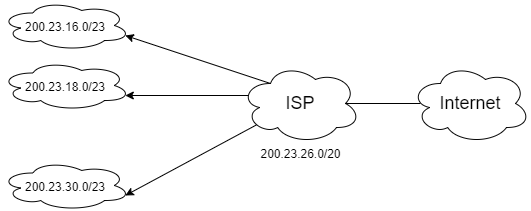
\includegraphics[width=300px]{images/5_Internetworking/hierarchical_addressing.png}
\end{figure}


\subsubsection{Ottenere un blocco di indirizzi}
Per ottenere un blocco di indirizzi ci si interfaccia con un Internet Service Provider, ogni ISP a sua volta chiede ad un ISP più grande e così via fino ad arrivare al provider di più alto livello che è ICANN - Internet Corporation for Assigned Names and Numbers.
Questa organizazione alloca gli indirizzi, gestisce i DNS ed assegna i nomi dei domini risolvendo eventuali dispute.

\subsubsection{Ottenere un indirizzo}
Un singolo host per avere un indirizzo può:
\begin{itemize}
    \item utilizzare un indirizzamento statico: si chiede al responsabile della rete la configurazione del singolo dispositivo
    \item utilizzare un indirizzamento dinamico: si utilizza un servizio della rete locale noto come DHCP - Dynamic Host Configuration Protocol che si occupa di assegnare gli IP agli host che lo richiedono utilizzando il protocollo stesso.
    Questa seconda via è plug-and-play in quanto basta che l' host si connetta alla rete e richieda in broadcast un indirizzo libero.
\end{itemize}

\subsection{DHCP}
E' il protocollo che permette di configurare i nuovi host che entrano nella rete.
La configurazione avviene tramite il così detto: \emph{four-way handshake} cioè uno scambio di 4 messaggi tra l' host che vuole configurarsi ed il server DHCP.
Questo scambio di messaggi è così operato:
\begin{itemize}
    \item il client invia in broadcast una richiesta "DHCP discover" nella quale richiede i servigi del server DHCP.
    In questa richiesta il client inserisce:
    \begin{itemize}
        \item come IP sorgente 0.0.0.0 porta 68
        \item come IP destinatario 255.255.255.255 porta 67
        \item come yiaddr (Your IP Address) 0.0.0.0
        \item inserisce un transaction ID generato casualmente
    \end{itemize}
    Essendo questo messaggio in broadcast tutti gli host nella sottorete lo ricevono, quindi anche un eventuale server DHCP

    \item il server risponde con un messaggio "DHCP offer" nel quale inserisce:
    \begin{itemize}
        \item come IP sorgente l'effettivo IP del server e porta 67
        \item come IP destinatario 255.255.255.255 porta 68
        \item come yiaddr l' indirizzo che si sta offrendo al client
        \item inserisce anche un lifetime cioè la durata temporale dell' associazione host-IP
        \item si inserisce lo stesso transaction ID che il client ha inserito
    \end{itemize}
    
    \item l' host risponde con un messaggio "DHCP request" nel quale inserisce:
    \begin{itemize}
        \item come IP sorgente 0.0.0.0 e porta 68
        \item come IP destinatario 255.255.255.255 e porta 67
        \item come yiaddr l' indirizzo IP che ha accettato
        \item come lifetime il lifetime ricevuto
        \item incrementa il transaction ID
    \end{itemize}
    Si noti che nonostante abbia accettato l' indirizzo la comunicazione continua sulla linea di broadcast
    
    \item il server risponde in fine con un messaggio "DHCP ACK" che è la copia del DHCP offer ma con il nuovo transaction ID.
    Anche questa risposta è fatta in broadcast.
\end{itemize}
Questo processo oltre ad assegnare un indirizzo IP assegna anche tutto il resto della configurazione, come ad esempio i server DNS da usare, la subnet mask ed il default gateway.

Prima che il lifetime scada un host può rinnovare la sua presenza e quindi l' associazione IP-host.
Questo lifetime è pensato per poter recuperare gli indirizzi non più utilizzati e poterli riassegnare, il tutto senza necessità che il client faccia sapere che si sta per disconnettere.

Il protocollo DHCP è un protocollo applicativo basato su UDP.

\subsection{NAT}
Il NAT - Network Address Translation è un meccanismo implementato nei router che permette di usare un solo indirizzo IP per connettere multipli host alla rete.
Sfruttiamo l' utilizzo di indirizzi IP privati, cioè che non sono routable, per nascondere una intera rete dietro un singolo indirizzo IP pubblico.
Tramite questo meccanismo possiamo usare meno indirizzi IP per rappresentare più host, possiamo cambiare gli indirizzi IP della rete privata senza modificare come appare l' host all' esterno della rete.
Possiamo cambiare ISP ed indirizzo IP pubblico senza modificare nulla nella configurazione dei singoli host nella rete privata, inoltre gli host nella rete privata non sono visibili dall' esterno quindi abbiamo anche un aumento della sicurezza.
\begin{figure}[H]
    \centering
    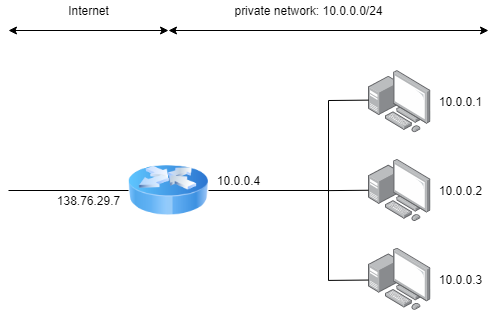
\includegraphics[width=300px]{images/5_Internetworking/NAT.png}
\end{figure}
La rete privata è 10.0.0.0/24, tra di loro gli host possono dialogare essendo nella stessa rete, per andare all' esterno serve qualcosa di più perché i loro indirizzi IP sono privati quindi il router si rifiuta di instradare pacchetti con quegli indirizzi IP.

Il NAT si occupa di sostituire l' IP sorgente privato con l' IP privato del router stesso, quindi quando 10.0.0.1 vuole dialogare con l' esterno invia datagrammi al router, il router sostituisce l' IP originale con 138.76.29.7 e provvede ad instradare il pacchetto sulla internet.

Per attuare questa traduzione il NAT usa una tabella interna di traduzione che associa all' indirizzo IP e porta del router esposta su internet l' indirizzo IP e porta dell' host interno alla rete.
Vediamo un esempio
\begin{itemize}
    \item 10.0.0.1 vuole trasmettere quindi crea un datagramma con 10.0.0.1:3345 e lo invia verso il router
    \item il router riceve il datagramma e sostituisce IP e porta con 138.76.29.7:5001 ed invia il datagramma verso internet.
    Inoltre aggiunge un record nella tabella in cui associa  138.76.29.7:5001 $<->$ 10.0.0.1:3345
    \item quando la rete risponde, risponde con un datagramma destinato a \\ 138.76.29.7:5001
    \item il router lo riceve, legge l' indirizzo IP, cerca nella sua tabella una entry con quell' indirizzo, la trova e traduce cambiando l' indirizzo IP in 10.0.0.1:3345 e provvede ad instradare il pacchetto nella rete locale.
\end{itemize}

Questo meccanismo come abbiamo visto funziona ed è molto elegante se è l' host interno alla rete a prendere l' iniziativa ed iniziare la comunicazione.
Se ad iniziare la comunicazione fosse un host nella Internet pubblica non potrebbe funzionare in quanto il NAT non è detto che abbia una entry che associ all' host interno alla rete.
Per risolvere questo problema si può ricorrere al port mapping cioè inserire manualmente delle righe nella tabella di traduzione in cui si associa una porta pubblica ad un host interno alla rete.
Questa tuttavia è una configurazione manuale permanente.

Un' altra soluzione è l' utilizzo dell'hole punching che non discuteremo.

Un' altra soluzione, utilizzata ad esempio da skype, è quella di passare per un host che è pubblico nella rete, detto relay, che mette in comunicazione i due host privati in maniera trasparente.

Questa traduzione fa uso delle porte del router, quindi abbiamo un limite massimo di oltre 60000 connessioni simultanee, che non è un grosso limite per le reti domestiche.
Un' altra controversia è quella che il router in mezzo, nonostante sia un dispositivo di layer 3, modifica informazioni del layer 4, quello di trasporto, quindi si sta violando la connessione end-to-end.
La soluzione migliore al problema sarebbe l' utilizzo di IPv6!

\subsection{Datagram forwarding}
\subsubsection{Forwarding nei router intermedi}
Se in una tabella di routing inserissimo singolarmente tutti gli host possibili avremmo una tabella troppo grande da poter gestire, la soluzione è memorizzare solamente gli indirizzi delle reti, dopodiché gli host nella stessa rete saranno tutti raggiungibili semplicemente instradando verso la sottorete.

Questa tabella quindi associa all' indirizzo di sottorete il prossimo hop al quale inoltrare il datagramma e l' interfaccia verso la quale si trova il next hop:
\begin{table}[ht!]
    \centering
    \begin{tabular}{l|l|l}
        Subnet Number & Next Hop & Interface \\
        \hline
        128.96.34.0/25 & Router R1 & interface 0 \\
        128.96.34.128/25 & Router R3 & interface 1 \\
        128.96.33.0/24 & Router R3 & interface 1 \\
    \end{tabular}
\end{table}

La codifica CIDR è comoda per noi umani che utilizziamo la notazione decimale, per i computer non lo è.
Nelle tabelle di forwarding quindi il CIDR viene memorizzato tramite una subnet mask che è un indirizzo scritto nella stessa notazione decimale puntata che però pone ad 1 i primi $x$ bit che compongono la porzione di rete.
Ad esempio una rete /24 ha la subnet mask 255.255.255.0, una /25 ha una subnet mask 255.255.255.128.

La tabella di forwarding è quindi meglio rappresentata da:
\begin{table}[ht!]
    \centering
    \begin{tabular}{l|l|l|l}
        Subnet Number & Subnet Mask & Next Hop & Interface \\
        \hline
        128.96.34.0 & 255.255.255.128 & Router R1 & interface 0 \\
        128.96.34.128 & 255.255.255.128 & Router R3 & interface 1 \\
        128.96.33.0 & 255.255.255.0 & Router R3 & interface 1 \\
    \end{tabular}
\end{table}

\begin{verbatim}
    DHost = Destination_IP_Address
    For each entry i in RoutingTable {
        DNet = (SubnetMask[i] & DHost)
        If(DNet == SubnetNumber[i]) {
            deliver datagram to NextHop[i] through Interface[i]
            break
        }
    }
\end{verbatim}

\subsubsection{Forwarding dall' host mittente}
Il mittente conosce il proprio indirizzo IP, la sua maschera di sottorete ed il suo default router, questo perché fa parte della configurazione di rete effettuata manualmente o tramite DHCP.
Se l' host deve inviare datagrammi ad un altro host e l' indirizzo IP destinatario è nella stessa rete allora lo invia direttamente, se l' IP destinatario è fuori dalla propria rete il datagramma è inviato verso il default router.
\begin{verbatim}
    SubnetNum = MySubnetMask & Dest_IP_Addr
    if(SubnetNum == MySubnetNum)
        deliver datagram to Dest_IP_Addr
    else
        forward datagram to default router
\end{verbatim}

\subsection{ARP}
Ogni volta che devo inoltrare un datagramma ad un qualsiasi host, che sia nella mia stessa rete o che sia fuori e quindi debba passare per il router, devo incapsulare il datagramma in un frame ethernet.
Per fare ciò devo conoscere l' indirizzo fisico dell' host destinatario o intermedio, ci serve quindi eseguire una traduzione degli indirizzi.
Il protocollo ARP - Address Resolution Protocol è utilizzato proprio per questo scopo.

L' host sorgente invia in broadcast una richiesta ARP contenente l' indirizzo IP del destinatario.
Essendo in broadcast tutti gli host della rete la ricevono, a questo punto il destinatario si accorge della richiesta e risponde con il proprio indirizzo fisico direttamente a chi gli ha fatto la richiesta, quindi non in broadcast.

Internamente agli host una cache mantiene le associazioni IP-MAC per un tempo ragionevole prima di cancellare l' associazione per evitare che l' informazione sia troppo vecchia e quindi obsoleta.

Questo protocollo è \emph{plug-and-play} in quanto non c'è bisogno dell'azione di nessuno affinché funzioni, è tutto automatico, nessuna configurazione da effettuare.

\subsection{ICMP}
Il protocollo ICMP - Internet Control Message Protocol è un protocollo usato da tutti gli host per inviare notifiche al livello di rete.
E' spesso utilizzato per notificare errori di qualche tipo al livello di rete, ma non solo.

Un messaggio ICMP si compone di:
\begin{itemize}
    \item un tipo
    \item un codice
    \item l' header ed i primi 8 byte di dati del datagramma IP che ha causato l' errore
\end{itemize}
Alcuni esempi sono:
\begin{table}[ht!]
    \centering
    \begin{tabular}{l|l|l}
        Tipo & Codice & Descrizione \\
        0 & 0 & Risposta all' echo \\
        3 & 0 & Rete di destinazione irragiungibile \\
        3 & 1 & Host di destinazione irragiungibile \\
        3 & 2 & Protocollo di destinazione non implementato \\
        3 & 3 & Porta di destinazione non aperta \\
        3 & 6 & Rete di destinazione sconosciuta \\
        3 & 7 & Host di destinazione sconosciuto \\
        8 & 0 & Richiesta echo \\
        9 & 0 & Router advertisement \\
        10 & 0 & Router discovery \\
        11 & 0 & TTL scaduto \\
        12 & 0 & Header IP errato \\
    \end{tabular}
\end{table}

NB: Il Router advertisement è la procedura effettuata dai router per dire alla rete che sono presenti e per spargere informazioni utili come ad esempio lo stato dei link ed il loro utilizzo.
Spesso queste informazioni sono utilizzate dagli altri router per costruire le proprie tabelle di routing o per aggiornare le proprie metriche.

NB: Il router discovery è il processo di ricerca dei router nelle vicinanze.

NB: I comandi ping e traceroute si basano sull' utilizzo di questo protocollo.

\subsection{IPv6}
Questa seconda versione del protocollo IP è stata creata per risolvere il problema della carenza degli indirizzi IP.
Inoltre ci sono altre motivazioni che spingono per il suo utilizzo come ad esempio:
\begin{itemize}
    \item il formato dell' header è pensato per rendere più veloce la processazione ed il forwarding dei datagrammi
    \item il formato dell' header è cambiato anche per facilitare la qualità del servizio
\end{itemize}
NB: IPv5 è un protocollo anch'esso - Internet Stream Protocol, per questo si ha il nome IPv6.

Il datagramma IPv6 prevede un header a dimensione fissa di 40 byte e non ammette la frammentazione.

\begin{figure}[H]
    \centering
    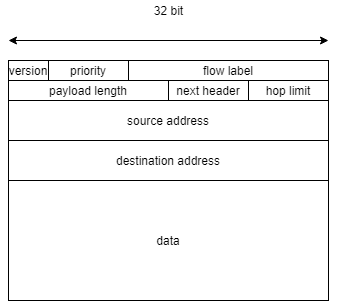
\includegraphics[width=200px]{images/5_Internetworking/IPv6_format.png}
\end{figure}
\begin{itemize}
    \item version: contiene sempre 6
    \item priority: indica la priorità del datagramma
    \item flow label: usato per identificare i datagrammi dello stesso flusso
    \item payload length: lunghezza in byte del campo dati
    \item next header: indica il protocollo del layer superiore
    \item hop limit: equivalente del TTL
\end{itemize}

NB: priority e flow label sono usati per gestire il QoS.

NB: non c'è un checksum per l' header, quindi non bisogna ricalcolarlo ogni volta che si decrementa hop limit.

Non essendoci frammentazione non possiamo inviare i datagrammi quando sono più grandi di MTU del media.
Questo significa che in caso ci sia questo problema si droppa del tutto il pacchetto e si invia un messaggio ICMP per notificare il mittente.
C'è anche una versione IPv6 di ICMP.

\subsubsection{Transizione da IPv4 ad IPv6}
Non essendoci la possibilità di passare da un giorno all' altro da un protocollo all' altro si sono applicate due soluzioni:
\begin{itemize}
    \item \emph{dual-stack}: i router implementano sia IPv4 che IPv6
    
    \item \emph{tunneling}: i datagrammi IPv6 vengono trasportati come dati all' interno di un datagramma IPv4 quando i router non possono dialogare nativamente IPv6:
    \begin{figure}[H]
        \centering
        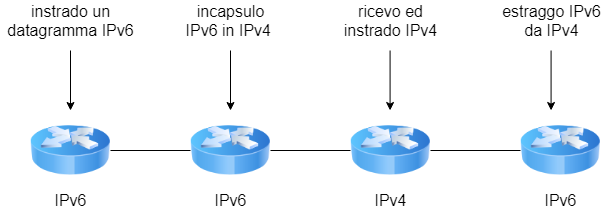
\includegraphics[width=300px]{images/5_Internetworking/ipv6_tunnelling.png}
    \end{figure}
\end{itemize}
